%package list
\documentclass{article}
\usepackage[top=3cm, bottom=3cm, outer=3cm, inner=3cm]{geometry}
\usepackage{graphicx}
\usepackage{url}
%\usepackage{cite}
\usepackage{hyperref}
\usepackage{array}
\usepackage{multicol}
\newcolumntype{x}[1]{>{\centering\arraybackslash\hspace{0pt}}p{#1}}
\usepackage{natbib}
\usepackage{pdfpages}
\usepackage{multirow}
\usepackage{float}
\usepackage[normalem]{ulem}
\useunder{\uline}{\ul}{}




%%%%%%%%%%%%%%%%%%%%%%%%%%%%%%%%%%%%%%%%%%%%%%%%%%%%%%%%%%%%%%%%%%%%%%%%%%%%
%%%%%%%%%%%%%%%%%%%%%%%%%%%%%%%%%%%%%%%%%%%%%%%%%%%%%%%%%%%%%%%%%%%%%%%%%%%%
\newcommand{\csemail}{vmachacaa@unsa.edu.pe}
\newcommand{\csdocente}{Vicente Machaca Arceda}
\newcommand{\cscurso}{Algoritmos y Estructura de Datos}
\newcommand{\csuniversidad}{Universidad Nacional de San Agustín}
\newcommand{\csescuela}{Maestría en Ciencia de la Computación}
\newcommand{\cspracnr}{01}
\newcommand{\cstema}{--}
%%%%%%%%%%%%%%%%%%%%%%%%%%%%%%%%%%%%%%%%%%%%%%%%%%%%%%%%%%%%%%%%%%%%%%%%%%%%
%%%%%%%%%%%%%%%%%%%%%%%%%%%%%%%%%%%%%%%%%%%%%%%%%%%%%%%%%%%%%%%%%%%%%%%%%%%%


\usepackage[english,spanish]{babel}
\usepackage[utf8]{inputenc}
\AtBeginDocument{\selectlanguage{spanish}}
\renewcommand{\figurename}{Figura}
\renewcommand{\refname}{Referencias}
\renewcommand{\tablename}{Tabla} %esto no funciona cuando se usa babel
\AtBeginDocument{%
	\renewcommand\tablename{Tabla}
}

\usepackage{fancyhdr}
\pagestyle{fancy}
\fancyhf{}
\setlength{\headheight}{30pt}
\renewcommand{\headrulewidth}{1pt}
\renewcommand{\footrulewidth}{1pt}
\fancyhead[L]{\raisebox{-0.2\height}{
\includegraphics[width=3cm]{img/logo_unsa}}}
\fancyhead[C]{}
\fancyhead[R]{\fontsize{7}{7}\selectfont	\csuniversidad \\ \csescuela \\ \textbf{\cscurso} }
\fancyfoot[L]{MSc. Vicente Machaca}
\fancyfoot[C]{\cscurso}
\fancyfoot[R]{Página \thepage}







\begin{document}
	
	\vspace*{10px}
	
	\begin{center}	
		\fontsize{17}{17} \textbf{ Práctica \cspracnr}
	\end{center}
	%\centerline{\textbf{\underline{\Large Título: Informe de revisión del estado del arte}}}
	%\vspace*{0.5cm}
	

	\begin{table}[h]
		\begin{tabular}{|x{4.7cm}|x{4.8cm}|x{4.8cm}|}
			\hline 
			\textbf{DOCENTE} & \textbf{CARRERA}  & \textbf{CURSO}   \\
			\hline 
			\csdocente & \csescuela & \cscurso    \\
			\hline 
		\end{tabular}
	\end{table}	
	
	
	\begin{table}[h]
		\begin{tabular}{|x{4.7cm}|x{4.8cm}|x{4.8cm}|}
			\hline 
			\textbf{PRÁCTICA} & \textbf{TEMA}  & \textbf{DURACIÓN}   \\
			\hline 
			\cspracnr & Algoritmos de ordenamiento  & 3 horas   \\
			\hline 
		\end{tabular}
	\end{table}
	
	
	\section{Datos de los estudiantes}
	Grupo: N° 8
	\begin{itemize}
		\item Integrantes: 
		\begin{itemize}
			\item Esai Josue Huaman Meza
			\item Alan Jerry Reyes Robles
			\item Jorge Luis Zegarra Guardamino
			\item Nestor Giraldo Calcinas Huaranga
		\end{itemize}		
	\end{itemize}
	
	
	
	
	
	
	\section{Introducción}
	
	Se hara un análisis comparativo 04 algoritmos de ordenamiento, buscando estudiar la complejidad de cada uno de estos y como las diferentes formas de resolver un mismo problema pueden afectar los tiempos de ejecución.
	
	Dado que para hacer un buen análisis se deben correr muchas pruebas, cree un par de scripts que me permitieran automatizarlas de forma tal que se pudieran correr de forma continua sin intervención. Se procura crear un pequeño ambiente controlado por lo que se usara una sola PC para reallizar las pruebas donde no estuvieran ejecutandose en paralelo otras tareas, dado que los tiempos de ejecución de cada prueba puede verse afectado al estar compartiendo recursos con otros procesos.

    En cada máquina se corrieron las pruebas con el mismo archivo de numeros aleatorios a ordenar, en intervalos de 100, luego de 1000 en 1000, luego de 10.000 en 10.000, hasta 50.000 de datos; estos resultados se guardaron en archivos CSV para poder visualizar luego con python.
	

	
	\section{Algoritmos de Ordenamiento}\label{sec:ejercicios}
	\begin{enumerate}
		\item Algoritmo Counting Sort
		
			Counting sort es un algoritmo de ordenación que ordena los elementos de una matriz contando el número de apariciones de cada elemento único de la matriz. El recuento se almacena en una matriz auxiliar y la clasificación se realiza asignando el recuento como un índice de la matriz auxiliar.
			
La clasificación de conteo se ejecuta en un conjunto de entrada relativamente más pequeño. Counting sort calcula, para cada elemento en el arreglo - X, el número de elementos que son menores que - X. Luego usa esta información para colocar X directamente en su posición en el arreglo ordenado.

La ordenación por selección toma dos arreglos adicionales.

\begin{itemize}
   \item Uno para el resultado, la matriz ordenada
   \item otro para almacenamiento temporal, donde el tamaño es   igual al número máximo en la matriz de entrada.
 \end{itemize}	
 
 Es interesante notar que este algoritmo no es un tipo de comparación. No verá ninguna comparación en el código. Este algoritmo utiliza valores de elementos para indexar en una matriz.
		
\begin{figure}[H]
\centering
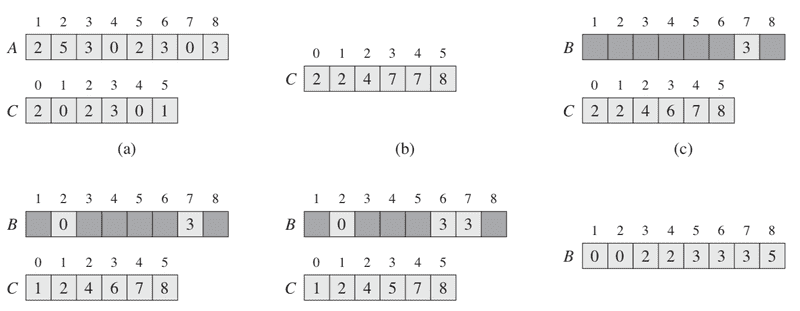
\includegraphics[width=0.7\textwidth]{img/CountS}
\caption{Algoritmo Counting Sort}
\label{fig:CountS}
\end{figure}


		
		Solución \\
		.................
		
		\item Algoritmo Heapsort
		
		Solución \\
		.................
\item Algoritmo Heapsort
		
		Solución \\
		.................

        \item \textbf{ALGORITMO MERGE SORT}
        
		 El algoritmo de ordenamiento por mezcla (merge sort) es un algoritmo de ordenamiento externo estable basado en la técnica divide y vencerás.
		 
        La idea de los algoritmos de ordenación por mezcla es dividir la matriz por la mitad una y otra vez hasta que cada pieza tenga solo un elemento de longitud. Luego esos elementos se vuelven a juntar (mezclados) en orden de clasificación.
        
        Conceptualmente, el ordenamiento por mezcla funciona de la siguiente manera: 
        \begin{itemize}
            \item Si la longitud de la lista es 0 o 1, entonces ya está ordenada.
        \end{itemize}
    
        En otro caso: 
        \begin{itemize}
            \item Dividir la lista desordenada en dos sublistas de aproximadamente la mitad del tamaño. 
            \item Ordenar cada sublista recursivamente aplicando el ordenamiento por mezcla. 
            \item Mezclar las dos sublistas en una sola lista ordenada.
        \end{itemize}

        El ordenamiento por mezcla incorpora dos ideas principales para mejorar su tiempo de ejecución:
        \begin{enumerate}
            \item Una lista pequeña necesitará menos pasos para ordenarse que una lista grande.
        \end{enumerate}
        \begin{enumerate}
            \item Se necesitan menos pasos para construir una lista ordenada a partir de dos listas también ordenadas, que a partir de dos listas desordenadas.
        \end{enumerate}
    
        
    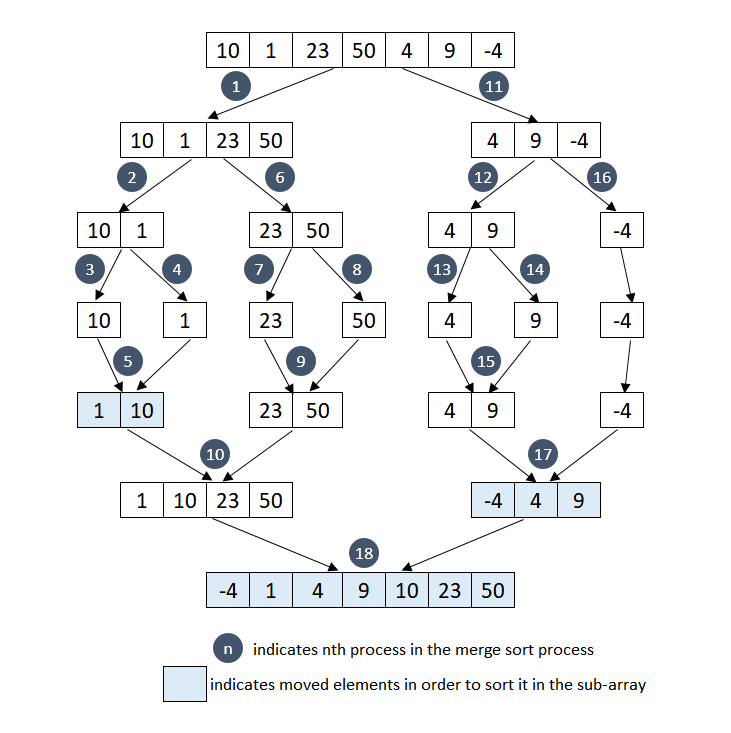
\includegraphics[width=\textwidth]{img/merge-sort}
        
        En todos los casos (el peor, el promedio y el mejor), el algoritmo Merge Sort siempre divide la matriz hasta que todas las submatrices contienen un solo elemento y tarda un tiempo lineal en fusionar esas submatrices. El proceso de división tiene una complejidad de tiempo $\Theta (logN)$ y el proceso de fusión tiene una complejidad de tiempo $\Theta (N)$. Por lo tanto, en todos los casos, la complejidad temporal del algoritmo Merge Sort es $\Theta(NlogN)$.

        Este tipo de ordenamiento es útil cuando se tiene una estructura ordenada y los nuevos datos a añadir se almacenan en una estructura temporal para después agregarlos a la estructura original de manera que vuelva a quedar ordenada
        
Merge sort es un ordenamiento estable, paraleliza mejor, y es más eficiente manejando medios secuenciales de acceso lento. Merge sort es a menudo la mejor opción para ordenar una lista enlazada: en esta situación es relativamente fácil implementar merge sort de manera que sólo requiera $\Theta (1)$ espacio extra, y el mal rendimiento de las listas enlazadas ante el acceso aleatorio hace que otros algoritmos (como quicksort) den un bajo rendimiento, y para otros (como heapsort) sea algo imposible.
	
		
	    \item Algoritmo Quicksort

		
	\end{enumerate}

\section{Implementación}

\section{Resultados}

    \begin{enumerate}
        \item Información del Sistema
        
        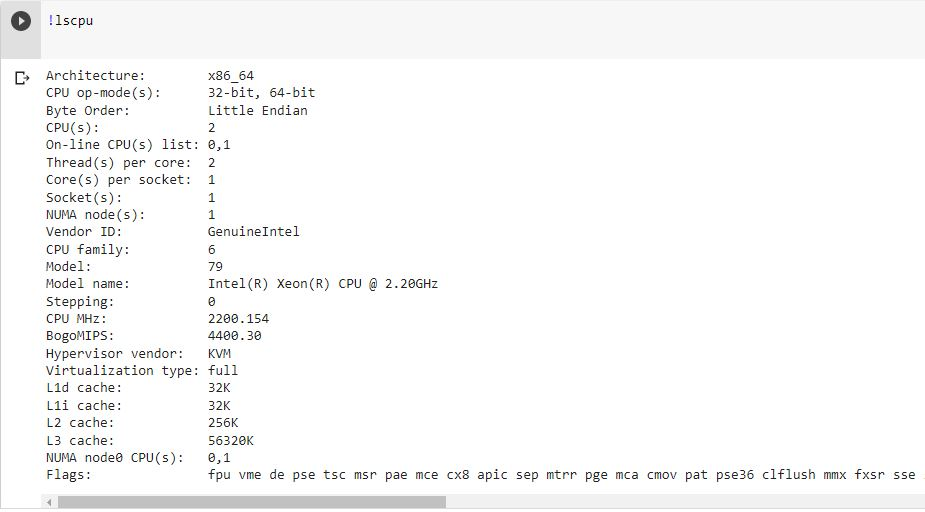
\includegraphics[width=\textwidth]{img/Captura1}
        
    \end{enumerate}

\section{Conclusiones}
	
	%\clearpage
	%\bibliographystyle{apalike}
	%\bibliographystyle{IEEEtranN}
	%\bibliography{bibliography}
		
	
\end{document}
